\documentclass[tikz,crop,preview, border=1cm, landscape]{standalone}

\def\meanOne{0.8}
\def\meanTwo{0.4}
\def\binOne{0.7}
\def\binTwo{0.44}
\def\binTwoStd{0.1}

\usepackage{pgfplots}
\pgfplotsset{compat=1.11}
\usepgfplotslibrary{fillbetween}
\begin{document}

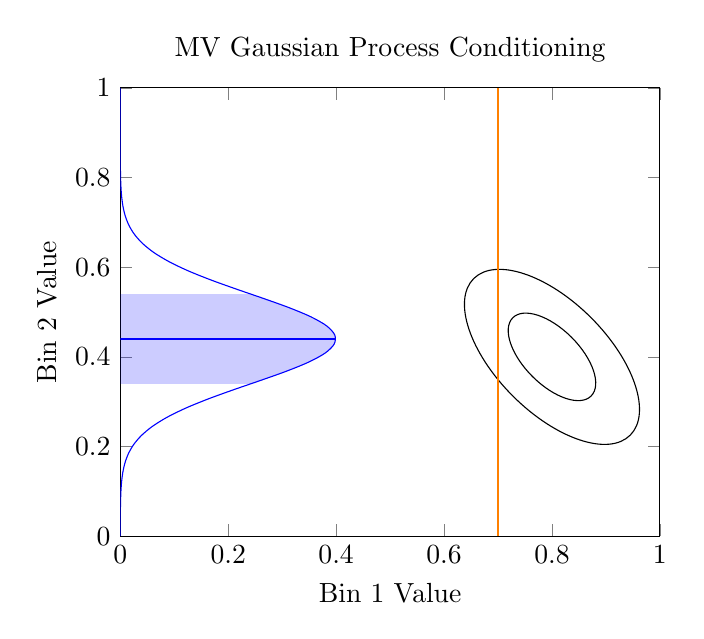
\begin{tikzpicture}
  \pgfmathdeclarefunction{gauss}{1}{%
    \pgfmathparse{1/(\binTwoStd*sqrt(2*pi))*exp(-((#1-\binTwo)^2)/(2*\binTwoStd^2))}%
  }
  \def\center{(axis cs: \meanOne,\meanTwo)} 
  \begin{axis}[
    ymin=0, ymax=1,
    xmin=0, xmax=1,
    xlabel={Bin 1 Value},
    ylabel={Bin 2 Value},
    title=MV Gaussian Process Conditioning]
    \draw[rotate around={45:\center}] \center ellipse (10pt and 20pt); 
    \draw[rotate around={45:\center},] \center ellipse (20pt and 40pt);
    \draw[thick,orange] (axis cs:\binOne,0) -- (axis cs:\binOne,1);

    \addplot+[name path=curve, draw=blue, domain=0:1,mark=none,samples=50,smooth]({ 0.1 * gauss(x)},{x});
    \draw[thick,blue] (axis cs: 0, \binTwo) -- (axis cs: {0.1 * gauss(\binTwo)}, \binTwo);

    \path[name path=yaxis] (axis cs:0,0) -- (axis cs:0,1);
    \path[name path=xaxis] (axis cs:0,0) -- (axis cs:1,0);
    \addplot+ [thick, color=blue, fill=blue, fill opacity=0.2]
    fill between[of=curve and yaxis,  soft clip={domain y=\binTwo+\binTwoStd:\binTwo-\binTwoStd}];
  \end{axis}
\end{tikzpicture}
\end{document}
